%%%%%%%%%%%%%%%%%%%%%%%%%%%%%%%%%%%%%%%
% Deedy - One Page Two Column Resume
% LaTeX Template
% Version 1.2 (16/9/2014)
%
% Original author:
% Debarghya Das (http://debarghyadas.com)
%
% Original repository:
% https://github.com/deedydas/Deedy-Resume
%
% IMPORTANT: THIS TEMPLATE NEEDS TO BE COMPILED WITH XeLaTeX
%
% This template uses several fonts not included with Windows/Linux by
% default. If you get compilation errors saying a font is missing, find the line
% on which the font is used and either change it to a font included with your
% operating system or comment the line out to use the default font.
% 
%%%%%%%%%%%%%%%%%%%%%%%%%%%%%%%%%%%%%%
% 
% TODO:
% 1. Integrate biber/bibtex for article citation under publications.
% 2. Figure out a smoother way for the document to flow onto the next page.
% 3. Add styling information for a "Projects/Hacks" section.
% 4. Add location/address information
% 5. Merge OpenFont and MacFonts as a single sty with options.
% 
%%%%%%%%%%%%%%%%%%%%%%%%%%%%%%%%%%%%%%
%
% CHANGELOG:
% v1.1:
% 1. Fixed several compilation bugs with \renewcommand
% 2. Got Open-source fonts (Windows/Linux support)
% 3. Added Last Updated
% 4. Move Title styling into .sty
% 5. Commented .sty file.
%
%%%%%%%%%%%%%%%%%%%%%%%%%%%%%%%%%%%%%%%
%
% Known Issues:
% 1. Overflows onto second page if any column's contents are more than the
% vertical limit
% 2. Hacky space on the first bullet point on the second column.
%
%%%%%%%%%%%%%%%%%%%%%%%%%%%%%%%%%%%%%%


\documentclass[]{deedy-resume-openfont}
\usepackage{fancyhdr}
\usepackage{graphicx}
\usepackage{paracol}
\columnratio{0.30}
\setlength{\columnsep}{0.04\textwidth}
\globalcounter{*}
    
\pagestyle{fancy}
\fancyhf{}
    
\begin{document}

%%%%%%%%%%%%%%%%%%%%%%%%%%%%%%%%%%%%%%
%
%     LAST UPDATED DATE
%
%%%%%%%%%%%%%%%%%%%%%%%%%%%%%%%%%%%%%%
\lastupdated

%%%%%%%%%%%%%%%%%%%%%%%%%%%%%%%%%%%%%%
%
%     TITLE NAME
%
%%%%%%%%%%%%%%%%%%%%%%%%%%%%%%%%%%%%%%
\namesection{张靖昊}{}{ 浙江杭州\ |\ 1997\ |\ \urlstyle{same}\href{mailto:zhang.jing.hao@outlook.com}{zhang.jing.hao@outlook.com} | 18645858867
}

%%%%%%%%%%%%%%%%%%%%%%%%%%%%%%%%%%%%%%
%
%     COLUMN ONE
%
%%%%%%%%%%%%%%%%%%%%%%%%%%%%%%%%%%%%%%

\begin{paracol}{2} 
\raggedright

%%%%%%%%%%%%%%%%%%%%%%%%%%%%%%%%%%%%%%
%     PHOTO
%%%%%%%%%%%%%%%%%%%%%%%%%%%%%%%%%%%%%%
{\centering
\raisebox{-\height}{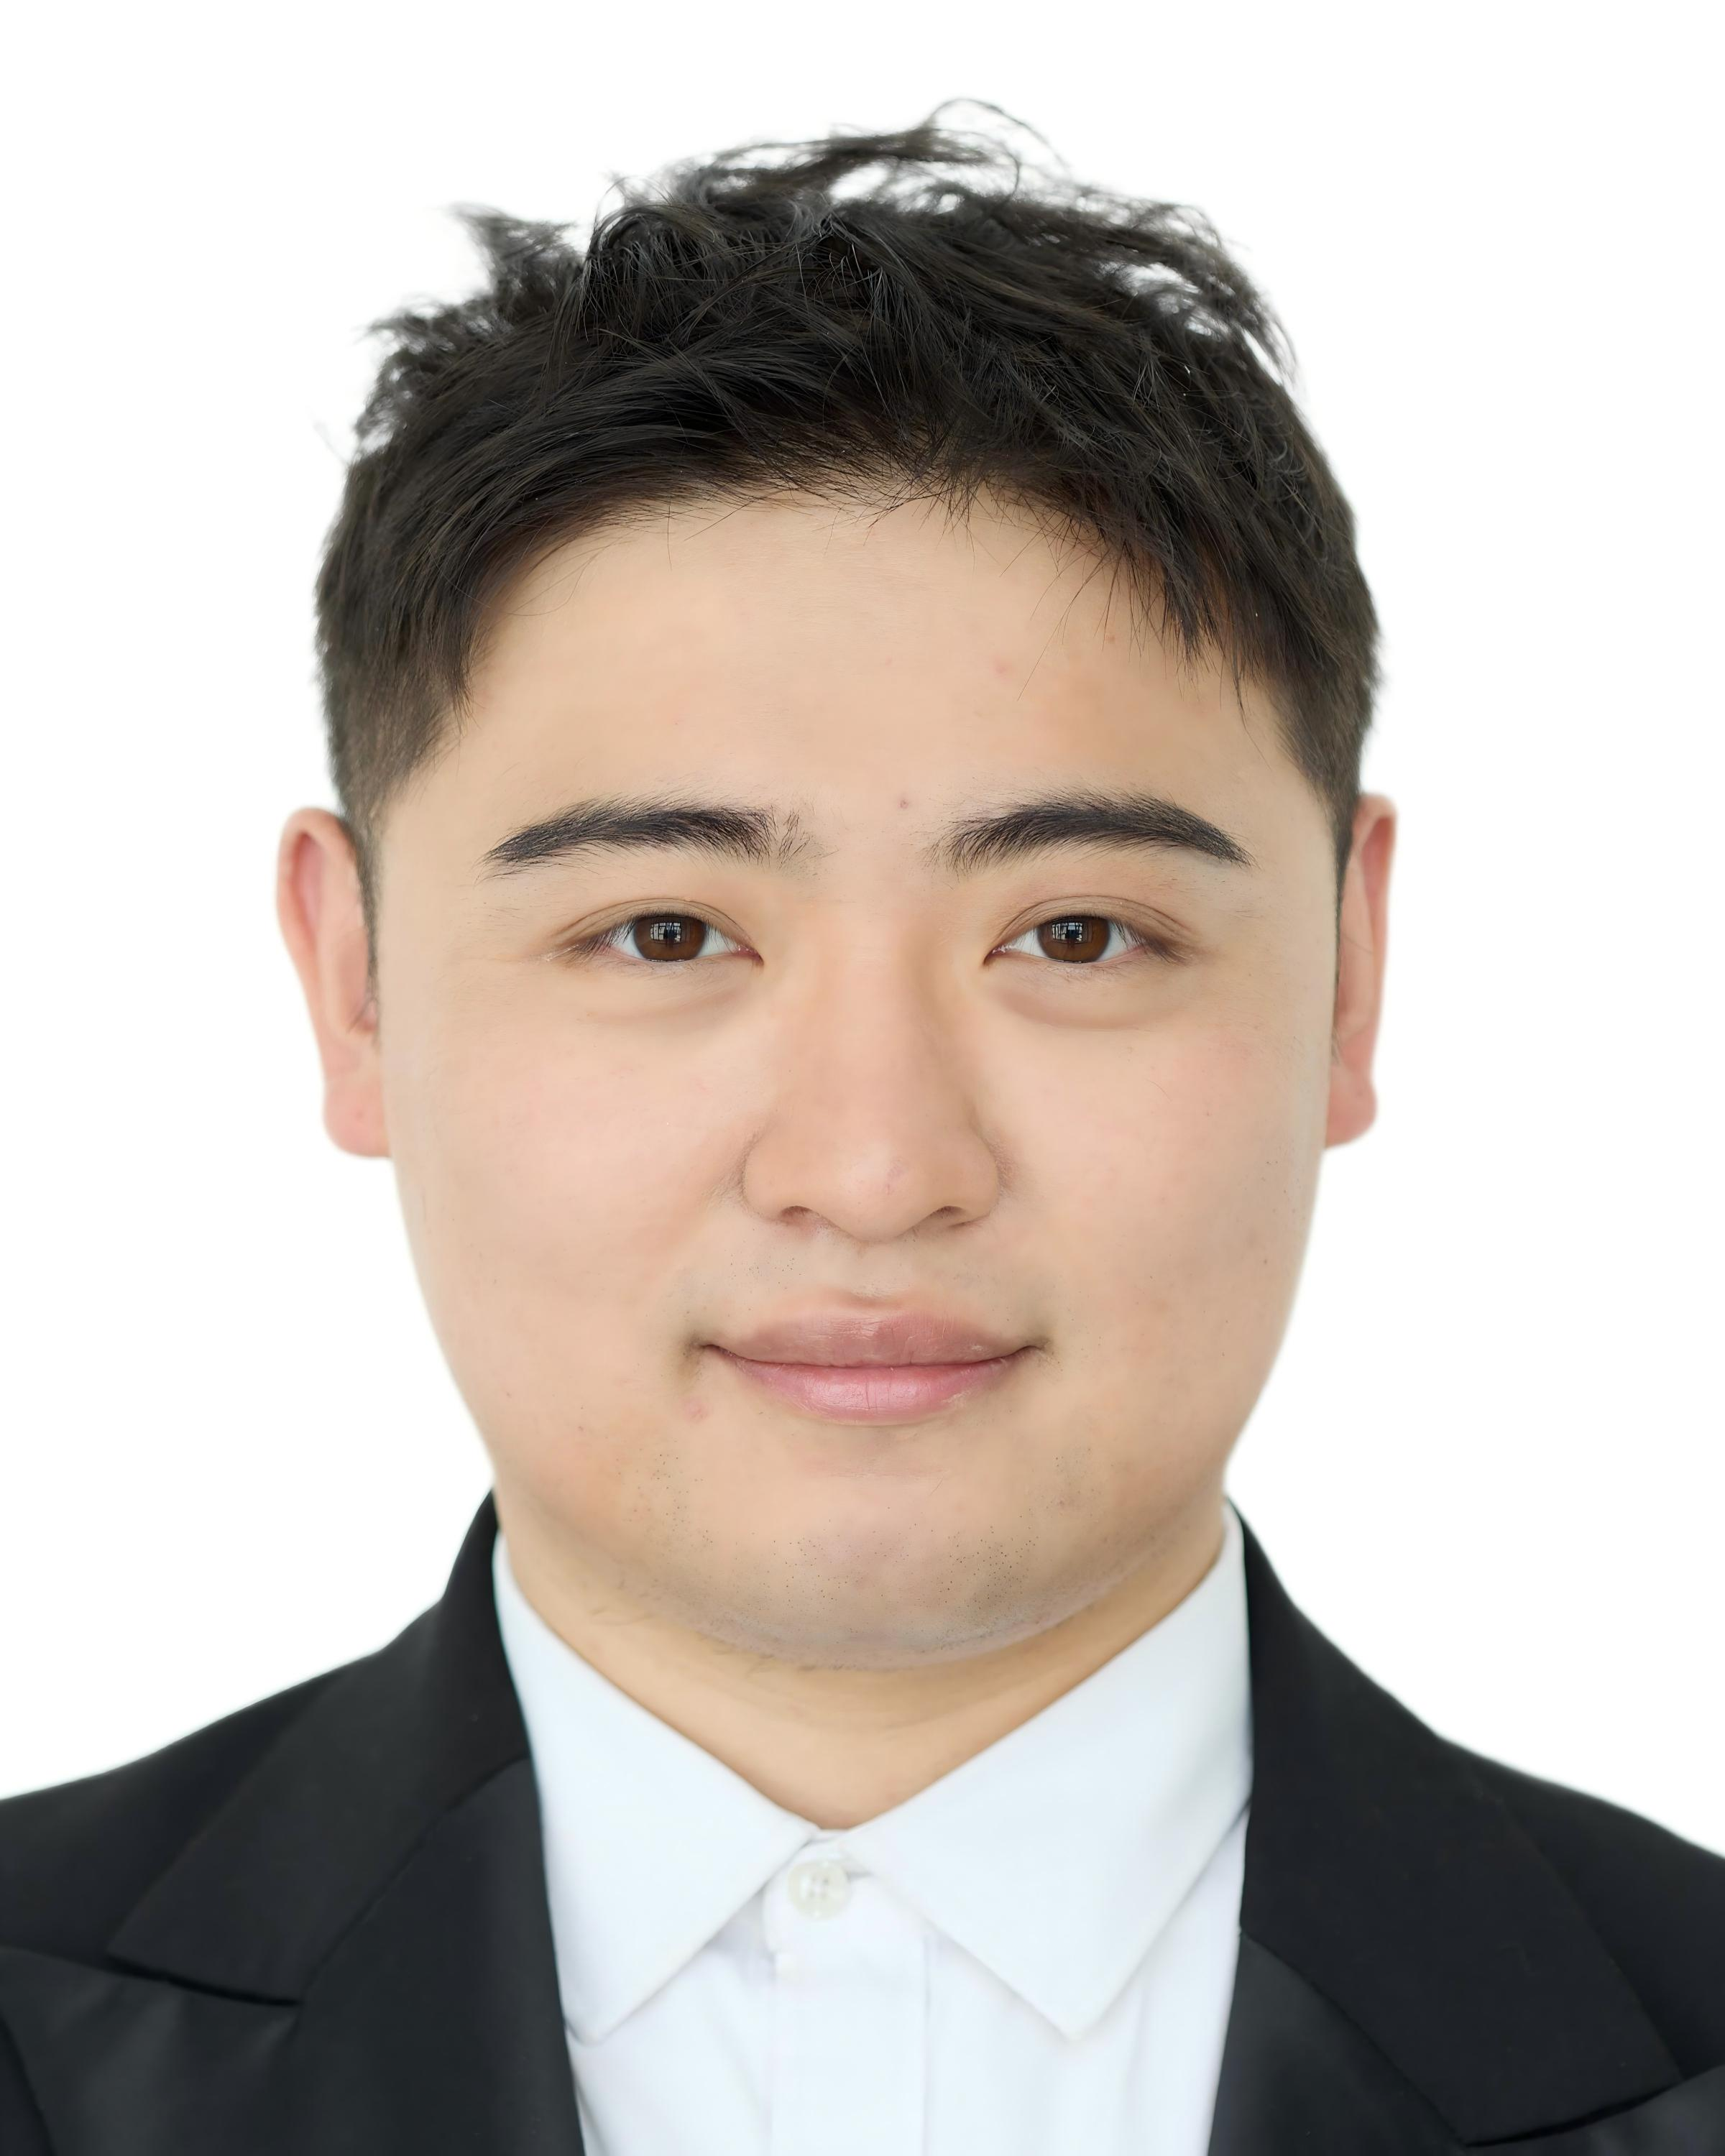
\includegraphics[height=3.4cm]{张靖昊照片.jpg}}\par}
\vspace{4pt}

%%%%%%%%%%%%%%%%%%%%%%%%%%%%%%%%%%%%%%
%     EDUCATION
%%%%%%%%%%%%%%%%%%%%%%%%%%%%%%%%%%%%%%

\section{教育经历} 

\subsection{悉尼科技大学}
\descript{University of Technology, Sydney}
\descript{软件工程（本科）}
\location{2017.10 - 2019.10}

\sectionsep

\subsection{哈尔滨工程大学}
\descript{Harbin Engineering University}
\descript{计算机科学与技术（本科）}
\location{2015.08 - 2019.07}

%%%%%%%%%%%%%%%%%%%%%%%%%%%%%%%%%%%%%%
%     LINKS
%%%%%%%%%%%%%%%%%%%%%%%%%%%%%%%%%%%%%%

% \section{链接}
% \sectionsep
% Gitee: \href{https://gitee.com/ZBeeeeeeeeee}{https://gitee.com/ZBeeeeeeeeee} \\
% GitHub: \href{https://github.com/zbeeeeeeeeee}{https://github.com/zbeeeeeeeeee} \\

%%%%%%%%%%%%%%%%%%%%%%%%%%%%%%%%%%%%%%
%     COURSEWORK
%%%%%%%%%%%%%%%%%%%%%%%%%%%%%%%%%%%%%%

% \section{修读课程}
% \subsection{Graduate}
% Advanced Machine Learning \\
% Open Source Software Engineering \\
% Advanced Interactive Graphics \\
% Compilers + Practicum \\
% Cloud Computing \\
% Evolutionary Computation \\
% Defending Computer Networks \\
% Machine Learning \\
% \sectionsep

%%%%%%%%%%%%%%%%%%%%%%%%%%%%%%%%%%%%%%
%     SKILLS
%%%%%%%%%%%%%%%%%%%%%%%%%%%%%%%%%%%%%%

\section{技能}

\subsection{AI 智能体}
Agent \textbullet{} 多 Agent 架构 \textbullet{} MCP \textbullet{} RAG \textbullet{} Skills \textbullet{} Function Calling \textbullet{} YOLO \textbullet{} OpenCV \textbullet{} 模型微调/量化/边缘部署 \\
\sectionsep

\subsection{软件架构 \& 后端}
\textbf{软件架构设计} \textbullet{} 微服务 \textbullet{} Java \textbullet{} Spring Boot \textbullet{} Node.js \textbullet{} RESTful API \textbullet{} 高并发 \\
\sectionsep

\subsection{数据库}
MySQL \textbullet{} PostgreSQL \textbullet{} Redis \\
\sectionsep

\subsection{应用开发}
鸿蒙（ArkTS）\textbullet{} Android（Java/Kotlin）\textbullet{} Flutter \textbullet{} Vue \textbullet{} Electron \\
\sectionsep

\subsection{嵌入式}
OpenHarmony \textbullet{} STM32 \textbullet{} GPIO \textbullet{} I2C \textbullet{} UART \textbullet{} MQTT \textbullet{} 传感器对接 \\
\sectionsep

\subsection{工具 \& 平台}
Git \textbullet{} Linux \textbullet{} Docker \textbullet{} Jenkins \textbullet{} Kubernetes \textbullet{} Postman \textbullet{} VS Code

%%%%%%%%%%%%%%%%%%%%%%%%%%%%%%%%%%%%%%
%     AWARDS
%%%%%%%%%%%%%%%%%%%%%%%%%%%%%%%%%%%%%%

\section{所获荣誉}

\textbullet{} 2025 华为 LCS 第一届 AI 应用开发大赛 TOP1 
\\
\textbullet{} 2023 浙江华为第七届最优秀讲师大赛 TOP1 
\\
\textbullet{} 2017 全美大学生数学建模大赛 Outstanding 奖 

%%%%%%%%%%%%%%%%%%%%%%%%%%%%%%%%%%%%%%
%
%     COLUMN TWO
%
%%%%%%%%%%%%%%%%%%%%%%%%%%%%%%%%%%%%%%

\switchcolumn
\raggedright

%%%%%%%%%%%%%%%%%%%%%%%%%%%%%%%%%%%%%%
%     EXPERIENCE
%%%%%%%%%%%%%%%%%%%%%%%%%%%%%%%%%%%%%%

\section{工作经历}
\sectionsep

\runsubsection{浙江华为通信技术有限公司}
\descript{AI 及软硬件开发工程师 | 金牌讲师}
\location{2021.01 - 至今 | 杭州}
\begin{tightemize}
    \item 主导多个 AI 及软硬件项目的全栈开发，覆盖需求分析、方案设计到交付上线的完整生命周期
    \item 作为公司\textbf{金牌讲师}，承担多个头部客户的培训任务，主导多门培训课程的设计与开发
    \item 跨团队协作推进项目交付，具备较强的项目管理与技术沟通能力
\end{tightemize}
\sectionsep

\runsubsection{同花顺}
\descript{移动应用开发工程师}
\location{2019.10 - 2020.12 | 杭州}
\begin{tightemize}
    \item 负责手机炒股 App 核心交易模块的设计与开发，支撑千万级用户交易场景
    \item 主导 AI 语音交易功能落地，参与移动端性能优化与架构迭代
\end{tightemize}
\sectionsep

%%%%%%%%%%%%%%%%%%%%%%%%%%%%%%%%%%%%%%
%     RESEARCH
%%%%%%%%%%%%%%%%%%%%%%%%%%%%%%%%%%%%%%

\section{培训项目经历}

\sectionsep

\runsubsection{待补充}
\descript{待补充}
\sectionsep

\section{研发项目经历}

\runsubsection{企业知识库智能问答 Agent 平台}
\descript{架构设计 \& 核心开发}
\location{2024.03 - 2024.11 | 华为}
\begin{tightemize}
    \item 主导基于\textbf{多 Agent + RAG}的企业级知识问答平台，覆盖文档接入、检索、生成的端到端链路
    \item 通过 \textbf{MCP} 协议接入内部工具，结合 Function Calling 实现工单查询、报表拉取等动作型任务调度
    \item 设计文档切片与混合检索策略，召回率提升 30\%，已服务 5+ 头部客户上线
\end{tightemize}
\sectionsep

\runsubsection{鸿蒙智能安防终端（端云协同）}
\descript{全栈开发}
\location{2022.06 - 2023.05 | 华为}
\begin{tightemize}
    \item 负责鸿蒙设备侧感知模块与 ArkTS 配套 App 的设计开发，打通端侧采集到云端治理链路
    \item 在设备侧部署 \textbf{YOLO + OpenCV} 轻量化目标检测，单帧推理压至 80ms 内
    \item 牵头完成多设备组网与近场发现联调，交付 demo 进入客户 PoC 验收
\end{tightemize}
\sectionsep

\runsubsection{AI 语音交易助手}
\descript{方案设计 \& 移动端开发}
\location{2020.03 - 2020.11 | 同花顺}
\begin{tightemize}
    \item 主导手机炒股 App 语音交易功能的方案设计，实现语音指令到下单全流程的端到端打通
    \item 基于意图识别 + 槽位提取将口语化指令映射为交易参数，识别准确率达 95\%
    \item 兼容千万级日活场景下的并发与风控校验，语音下单转化率提升 12\%
\end{tightemize}
\sectionsep

\runsubsection{华为培训业务中台（微服务架构）}
\descript{架构设计 \& 后端开发}
\location{2021.06 - 2022.03 | 华为}
\begin{tightemize}
    \item 主导培训业务中台的\textbf{微服务架构设计}，基于 Spring Boot 拆分课程、排课、考核等服务
    \item 设计 MySQL + PostgreSQL 混合存储与读写分离方案，核心接口延迟压至 100ms 内
    \item 沉淀服务治理与接口规范，新业务接入周期缩短约 40\%
\end{tightemize}
\sectionsep

\runsubsection{AI 应用开发实训与评测平台}
\descript{全栈开发}
\location{2022.09 - 2023.02 | 华为}
\begin{tightemize}
    \item 基于 Node.js + Vue 搭建在线实训与评测平台，支撑内部 AI 应用开发大赛的提交与自动评分
    \item 设计可插拔评测调度与多语言沙箱架构，稳定承载千人级并发
\end{tightemize}
\vspace{2pt}

%%%%%%%%%%%%%%%%%%%%%%%%%%%%%%%%%%%%%%
%     PUBLICATIONS
%%%%%%%%%%%%%%%%%%%%%%%%%%%%%%%%%%%%%%

% \section{Publications} 
% \renewcommand\refname{\vskip -1.5cm} % Couldn't get this working from the .cls file
% \bibliographystyle{abbrv}
% \bibliography{publications}
% \nocite{*}

\end{paracol}
\end{document}  \documentclass[]{article}
